{\large \bf Task 2}
\begin{enumerate}
    %1.
  \item Machine learning is the study of finding or making a function $f$ that takes input $x$(feature vector) from some set $D$ and gives output $y$, where nothing is known about the relationship between $x$ and $y$ a priori.
        Supervised learning is the case where $y$ is known for some subset of $D$.
        Unsupervised learning is the case where nothing is known about the ouput of the function.
        An example would be taking a picture, $x$, of a dog or cat and finding a function, $f$, to classify the picture as a picture of a dog or cat, $y$.
  %2.
  \item
      \begin{enumerate}
        \item Feature scaling is changing the values of (numeric)features so that they conform to some restriction, without significantly changing the information encoded within the features.
        \item Distance based learning algorithms.
          \begin{itemize}
            \item K Nearest Neighbors
            \item Neural networks
            \item State Vector Machines
          \end{itemize}
        \item Tree and ensemble based algorithms
          \begin{itemize}
            \item Random forest
            \item XGB
          \end{itemize}
      \end{enumerate}
  %3.
    \item
      \begin{enumerate}
        \item
          \begin{minipage}[t]{0.9\textwidth}
            \centering
            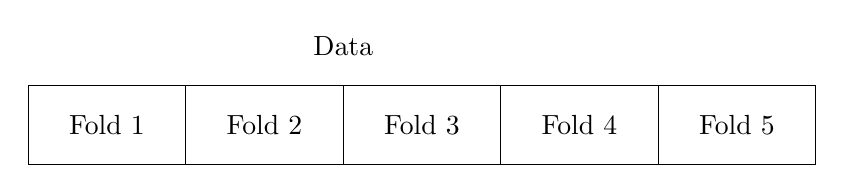
\begin{tikzpicture}[baseline=(current bounding box.north)]
              \draw[] (4,1.5) node {Data};
              \draw (0,0) -- (0,1) -- (10,1) -- (10,0) -- (0,0);
              \draw[] (1,0.5) node {Fold 1};
              \draw (2,0) -- (2,1);
              \draw[] (3,0.5) node {Fold 2};
              \draw (4,0) -- (4,1);
              \draw[] (5,0.5) node {Fold 3};
              \draw (6,0) -- (6,1);
              \draw[] (7,0.5) node {Fold 4};
              \draw (8,0) -- (8,1);
              \draw[] (9,0.5) node {Fold 5};
            \end{tikzpicture}\\
            $\phantom{a.}$\\
          \end{minipage}\\
          The feature/training data set is partitioned into various folds, as seen in the diagram above for five folds.
          The cross validation iterates through the partitions.
          For each iteration one fold is chosen as a test set and the other partitions are grouped into one training set.
          The cross validation then trains a model on the training partitions and evaluates the trained model on the test partition.
          This gives an estimate of generalization error of the model.
        \item
          Large number of folds:
          \begin{description}
              \item[Pro] Bias of true error rate is small.
              \item[Con] Computationally expensive.
              \item[Con] Large variance in estimator.
          \end{description}
          Small number of folds:
          \begin{description}
              \item[Pro] Computationally cheaper than large number of folds.
              \item[Pro] Low variance of estimator.
              \item[Con] Error estimator has high bias.
          \end{description}
      \end{enumerate}
    %4
    \item
      \begin{enumerate}
          \item
            Gradient descent tries to find the minimum in some function, see the figure below.\\
            \begin{minipage}[t]{0.95\textwidth}
              \begin{center}
                \includegraphics[scale = 0.75]{task2/gradDesc.jpg}

                From \url{https://www.researchgate.net/figure/Gradient-Descent-Algorithm-26_fig1_352019480}\\
              \end{center}
              $\phantom{a.}$\\
            \end{minipage}
            This is used in machine learning to minimize a cost function, the cost function should be low when the machine learning model performs well and high when the model performs badly.
            The gradient descent method finds the direction in which the cost function decreases the fastest, and takes a step in that direction.
            The gradient descent method might only find a (poor) local minimum and not the global minimum.
            The gradient descent method might also find a saddle point in the cost function, see black dot in the figure below.\\
            \begin{center}
            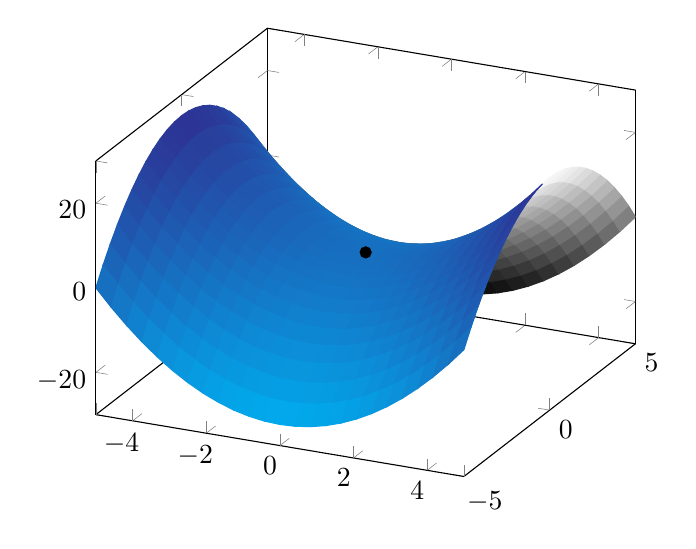
\begin{tikzpicture}
              \begin{axis}
                \addplot3 [color=black, draw=none, mark=*, mark size=2]
                table[row sep=crcr] {%
                0 0 0\\
                };
                \addplot3 [surf,
                  mesh/interior colormap={blueblack}{
                  color=(cyan) color=(blue)
                  },
                  colormap/blackwhite,
                  shader=flat] {x^2-y^2};
              \end{axis}
            \end{tikzpicture}
            \end{center}
            A potential solution to this problem is to find a cost function with one minimum, but this could be very complicated, if not impossible, for a particular problem.
            Another problem is that one has to worry about setting a learning rate for model updates. 
            Small learning rates result in slow solution and high learning rates can miss the minima in the cost function.
            This can be solved by giving the gradient descent solver a momentum which essentially adaptively modifies the learning rate to a suitable value.
          \item
            By looking at the error data, overfitting and underfitting of the model can be seen.
            If the error of the model on training data decreases, but the generalization error increases the model is overfitting.
            If the model has a high overall error on both training and test sets, and the error does not decrease with training, the model is probably too simple and so underfits.
            If the model is overfitting then the model is too complex, a lower degree polynomial is required.
            If the model is underfitting the model is too simple and a higher order polynomial is required.

          \item
            By looking at the error data, overfitting and underfitting of the model can be seen.
            If the model is overfitting then more regularization is needed.
            If the model is starting to underfit then less regularization is needed.
      \end{enumerate}
\end{enumerate}
